\section{Appendix}
\subsection{Double and Triple Integrals}
The \textbf{three types} of \textbf{simple domains of integration} are,

\begin{defn}[Type I]
	A \textbf{Type I} domain of integration is,
	\begin{center}
    
\includegraphics[width=0.7\linewidth]{figures/wk-6/type-1.png}
    \end{center}
\end{defn}

\begin{defn}[Type II]
	A \textbf{Type II} domain of integration is,
	\begin{center}
    
\includegraphics[width=0.7\linewidth]{figures/wk-6/type-2.png}
    \end{center}
\end{defn}
	
\begin{defn}[Type III]
	A \textbf{Type III} domain of integration is,
	\begin{center}
    
\includegraphics[width=0.7\linewidth]{figures/wk-6/type-3.png}
    \end{center}
\end{defn}

\begin{rmk}
    To compute a \textbf{triple integral},
    \[\iiint_D f(x, y, z) d x d y d z\]
    we decompose $D$ into simple domains of integration,
    \[\int_{x=a}^{x=b}\left[\int_{y=l_1(x)}^{y=l_2(x)}\left[\int_{z=\Psi_1(x, y)}^{z=\Psi_2(x, y)} f(x, y, z) d z\right] d y\right] d x\]
\end{rmk}

\begin{marginfigure}
        \begin{center}
        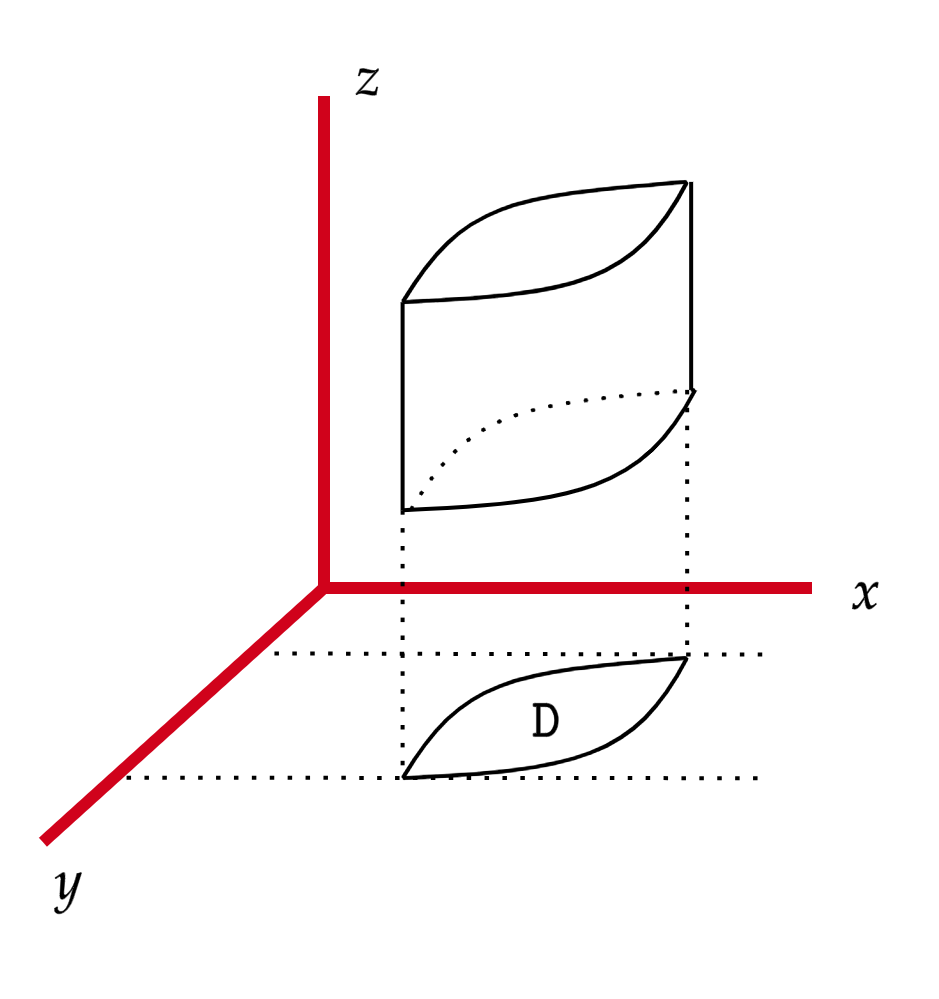
\includegraphics[width=\linewidth]{figures/wk-6/type-4.png}
        \end{center}
\end{marginfigure}

\begin{ex}{$\iint_D(x+2 y) d x d y$}{label}
	We will compute $\iint_D(x+2 y) d x d y$ over a Type I domain.
	\begin{center}
    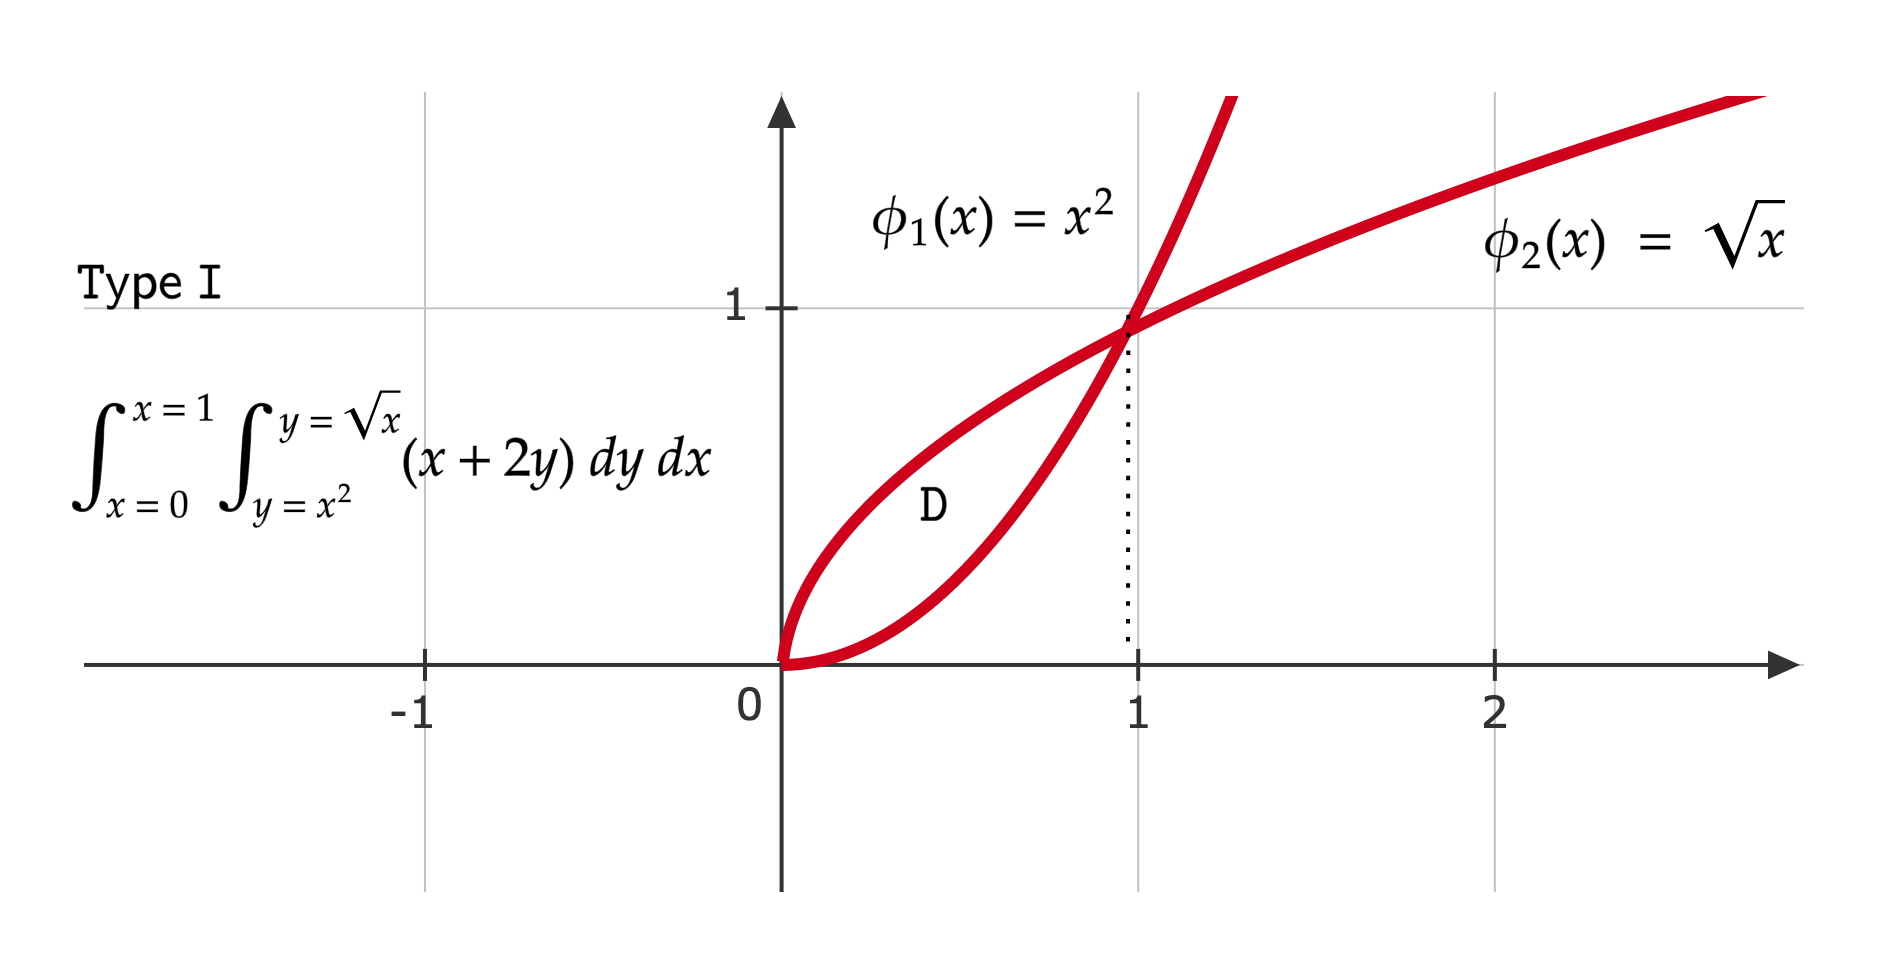
\includegraphics[width=\linewidth]{figures/wk-6/fig-8.png}
    \end{center}
    In this case,
    \begin{align*}
    	\int_{x=0}^{x=1}\left[\int_{y=x^2}^{y=\sqrt{x}}(x+2 y) d y\right] d x
    	&=\int_{x=0}^{x=1}\left[x y+y^2\right]_{y=x^2}^{y=\sqrt{x}} d x \\
    	&= \int_{x=0}^{x=1} x^{3 / 2}-x^3+x-x^4 d x \\
    	&= 9/20
    \end{align*}
    We can also compute $\iint_D(x+2 y) d x d y$ over a Type II domain.
    \begin{center}
    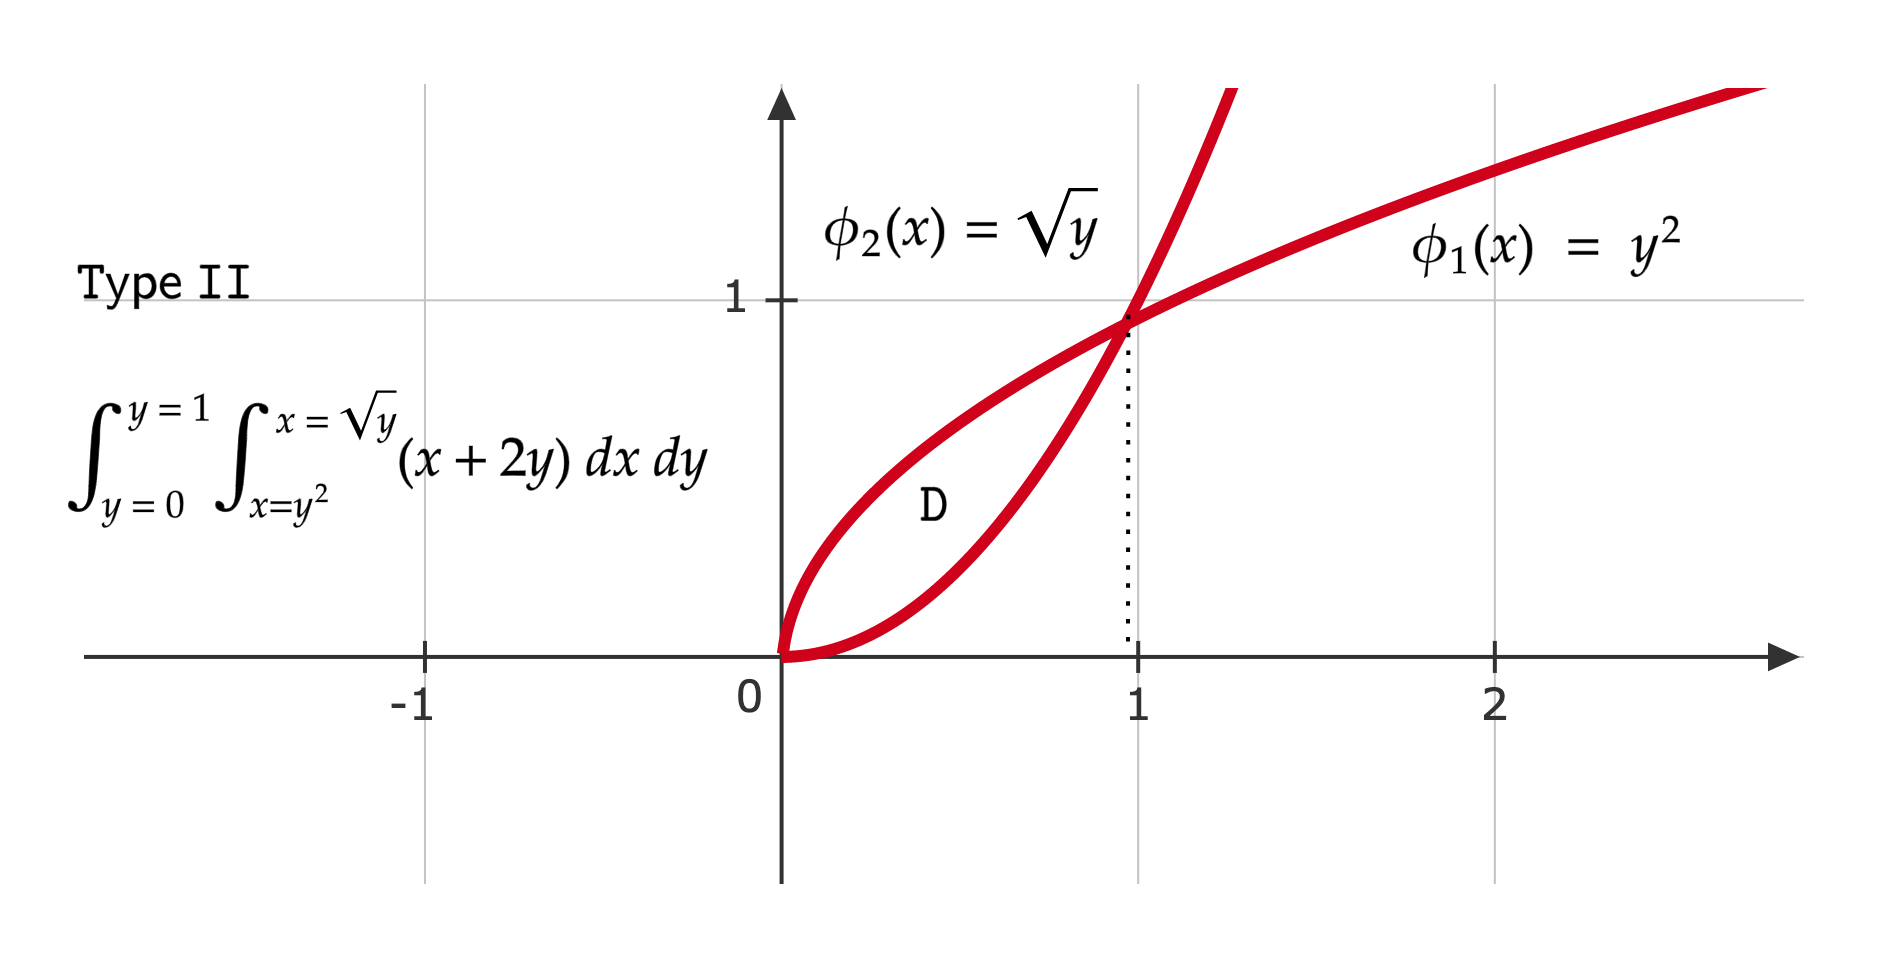
\includegraphics[width=\linewidth]{figures/wk-6/fig-9.png}
    \end{center}
\end{ex}

\begin{ex}{Volume of a Sphere of Radius $r$}{label}
	The formula for the volume of a sphere is
	\[8 \int_{x=0}^{x=r}\left[\int_{y=0}^{y=\sqrt{r^2-x^2}}\left[\int_{z=0}^{z=\sqrt{r^2-x^2-y^2}} d z\right] d y\right] d x = \frac{4}{3} \pi r^2\]
\end{ex}

\subsection{Change of Variables}
The formula for \textbf{change of variables} for simple integrals is,
\begin{thm}
    Under the following conditions,
    \begin{enumerate}
        \item $f$ is continuous
        \item $u \mapsto x(u)$ is continuously differentiable on $[a,b]$
    \end{enumerate}
    we can relate the two integrals,
    \[\int_a^b f(x(u)) \frac{d x}{d u}(u) \cdot d u = \int_{x(a)}^{x(b)} f(x) dx\]
\end{thm}

\noindent Suppose that $u \mapsto x(u)$ is one-to-one on $[a,b] := I^*$. Let $I$ be the interval whose endpoints are given by $x(a)$ and $x(b)$. That is,
\[I=\begin{cases}
    [x(a), x(b)] & x \text { is increasing } \iff x_u(u) \geq 0 \text{ on } [a,b] \\
    [x(b), x(a)] & x \text { is decreasing } \iff x_u(u) \geq 0 \text{ on } [a,b]
\end{cases}\]
If $x_u(u) \geq 0 \text{ on } [a,b]$, then,
\[\int_a^b f(x(u)) \frac{d x}{d u}(u) \cdot d u = \int_{x(a)}^{x(b)} f(x) dx\]
Otherwise,
\[\int_a^b f(x(u)) \frac{d x}{d u}(u) \cdot d u = -\int_{x(a)}^{x(b)} f(x) dx\]
We combine these to obtain,
\[\int_{I^*} f(x(u))\left|\frac{d x}{d u}(u)\right| d u=\int f(x) d x\]
where the absolute value covers both cases.

\begin{thm}
    If $T: A^* \subseteq \R^2 \rightarrow A \subseteq \R^2$ is bijective and $C^1$, then,
    \[\iint_{A = T(A^*)} f(x,y) dx dy = \iint_{A^*}f(x(u,v), y(u,v)) \left|\frac{\partial(x, y)}{\partial(u, v)}\right| d u d v\]
    where 
    \[\frac{\partial(x, y)}{\partial(u, v)} = \operatorname{det}\underbrace{\left(\begin{array}{ll}
x_u & x_v \\
y_u & y_v
\end{array}\right)}_{(\mathbf{D}(T))}\]
is the determinant of the Jacobian matrix of $T$.
\end{thm}

\begin{rmk}
    By properties of the determinant,
    \[\frac{\partial(u, v)}{\partial(x, y)}=\mathbf{D}(T^{-1}) = (\mathbf{D}(T))^{-1}=\frac{1}{\frac{\partial(x, y)}{\partial(u, v)}}\]
\end{rmk}

\begin{rmk}
    If $T: A^* \rightarrow A$ maps $\partial A^*$ to $\partial A$ in a one-to-one and onto fashion at $\text{det}(\mathbf{D})(T) \neq 0$, then $T$ is one-to-one and onto.
\end{rmk}

\begin{ex}{$\iint(x+y) d x d y$}{label}
    We will compute $\iint_A (x+y) d x d y$ where
    \[A = \{(x, y) \in \R^2 \mid 0 \leq y \leq x \text{ and } 0 \leq x \leq 1\}\]
    Define the transformation
    \[T:(u, v) \longmapsto \left\{\begin{aligned}
    &x(u, v)=u+v \quad \quad \implies u = \frac{x+y}{2}\\
    &y(u, v)=u-v \quad \quad \implies v = \frac{x-y}{2}
    \end{aligned}\right.\]
    \begin{center}
    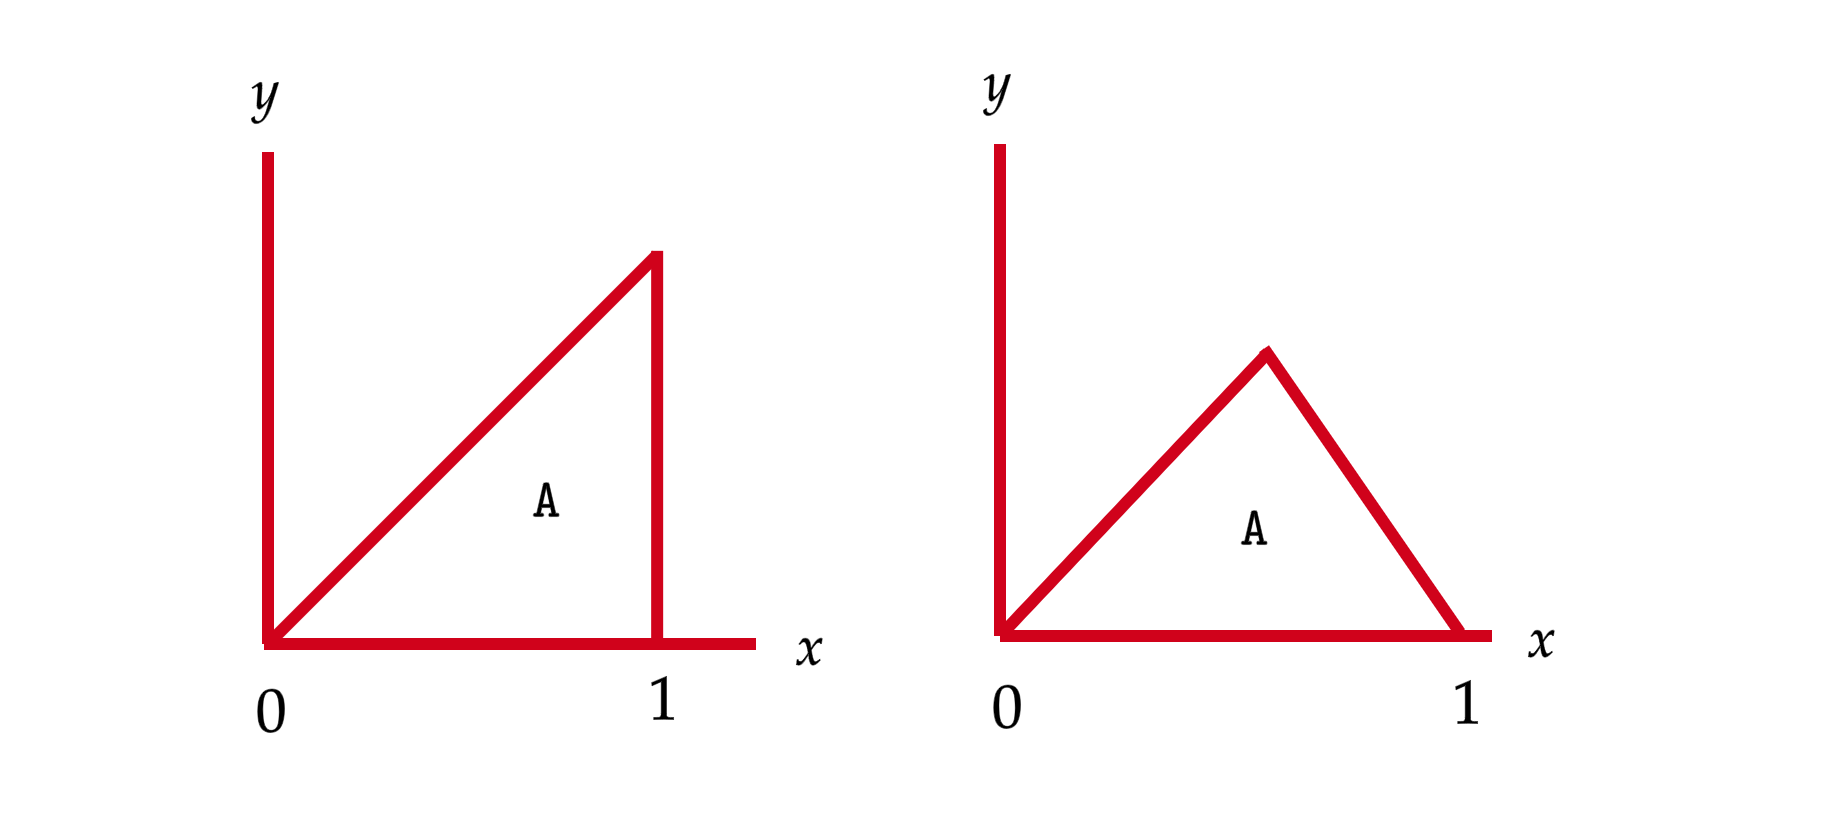
\includegraphics[width=0.7\linewidth]{figures/wk-6/fig-10.png}
    \end{center}
    We first calculate the determinant of the Jacobian,
    \[\frac{\partial(x, y)}{\partial(u, v)}=\operatorname{det}\left(\begin{array}{ll}
    x_u & x_v \\
    y_u & y_v
    \end{array}\right) = \operatorname{det}\left(\begin{array}{cc}
    1 & 1 \\
    1 & -1
    \end{array}\right)\]
    which gives the integral,
    \[\iint_{A^*} 2u \cdot 2 du dv = \int_{v=0}^{v=1} \int_{u=v}^{u=1-v} 2u \cdot 2 du dv = \frac{1}{2}\]
    where $x + y = 2u$ by our choice of $x = u + v$ and $y = u - v$.
\end{ex}

\begin{ex}{$\iint_A\left(1+x^2+y^2\right)^{3 / 2} d x d y$}{label}
    We will compute $\iint_A\left(1+x^2+y^2\right)^{3 / 2} d x d y$ where $A$ is the unit disk in the $x-y$ plane. Define the transformation,
    \[T:(r, \theta) \longmapsto(x=r \cos \theta, y=r \sin \theta)\]
    We begin by writing $A$ in polar coordinates,
    \[\{(r, \theta) \in \mathbb{R}^2 \mid 0 \leq r \leq 1 \text{ and } 0 \leq \theta \leq 2 \pi\}\]
    The determinant of the Jacobian matrix is,
    \[(\mathbf{D})(T)=\left(\begin{array}{ll}
    x_r & x_\theta \\
    y_r & y_\sigma
    \end{array}\right)=\left(\begin{array}{cc}
    \cos \theta & -r \sin \theta \\
    \sin \theta & r \cos \theta
    \end{array}\right)\]
    which implies that,
    \[\frac{\partial(x, y)}{\partial(r, \theta)} = r \cos ^2 \theta+ r \sin ^2 \theta = r\]
    It follows that the desired integral is,
    \begin{align*}
        \iint_{A^*}\left(1+r^2\right)^{3 / 2} r d r d \theta
        &= \int_{\theta = 0}^{\theta = 2\pi} \int_{r = 0}^{r = 1} (1 + r^2)^{3/2} r d r d \theta \\
        &= 2 \pi \int_{1}^{2} u^{3/2}\frac{1}{2} du \\
        &= \frac{2 \pi}{5}(4 \sqrt{2}-1)
    \end{align*}
    
\end{ex}

\begin{thm}
    If $T: A^* \subseteq \R^3 \rightarrow A \subseteq \R^3$ is bijective and $C^1$, then,
    \[\iiint_{A = T(A^*)} f(x,y, z) dx dy dz\]
    is equal to the integral,
    \[= \iiint_{A^*}f(x(u,v, w), y(u,v, w), z(u, v, w)) \left|\frac{\partial(x, y, z)}{\partial(u, v, w)}\right| d u d v d w\]
\end{thm}

\subsection{Spherical and Cylindrical Coordinates}
\noindent \textbf{Cylindrical coordinates} involve the transformation,
\begin{center}
    
\includegraphics[width=0.7\linewidth]{figures/wk-6/fig-11.png}
\end{center}
with the determinant,
\[\frac{\partial(x, y, z)}{\partial(r, \theta, z)}=\left(\begin{array}{lll}
x_r & x_\theta & x_z \\
y_r & y_q & y_z \\
z_r & z_\theta & z_z
\end{array}\right) =\left(\begin{array}{ccc}
\cos \theta & -r \sin \theta & 0 \\
\sin \theta & r \cos \theta & 0 \\
0 & 0 & 1
\end{array}\right) = r\]

\begin{ex}{$\iiint_A\left(x^2+y^2+z^2\right) d x d y d z$}{label}
    We will use cylindrical coordinates to compute the integral
    \[\iiint_A\left(x^2+y^2+z^2\right) d x d y d z\]
    along the $z$ axis, where,
    \[A = \{(x, y, z) \mid x^2+y^2 \leq 2 \text{ and } -2 \leq z \leq 3\}\]
    Applying the change of variables formula,
    \[\iiint_{A^*} (r^2 \cos^2 \theta + r^2 \sin^2 \theta + z^2) r dr d\theta dz\]
    We obtain that,
    \[\int_{\theta = 0}^{\theta = 2 \pi} \int_{z = -2}^{z = 3} \int_{r = 0}^{r = \sqrt{2}} (r^2 + z^2) r dr dz d \theta = \pi \cdot \frac{100}{3}\]
\end{ex}

\textbf{Spherical coordinates} involve the transofmration,
\begin{center}
    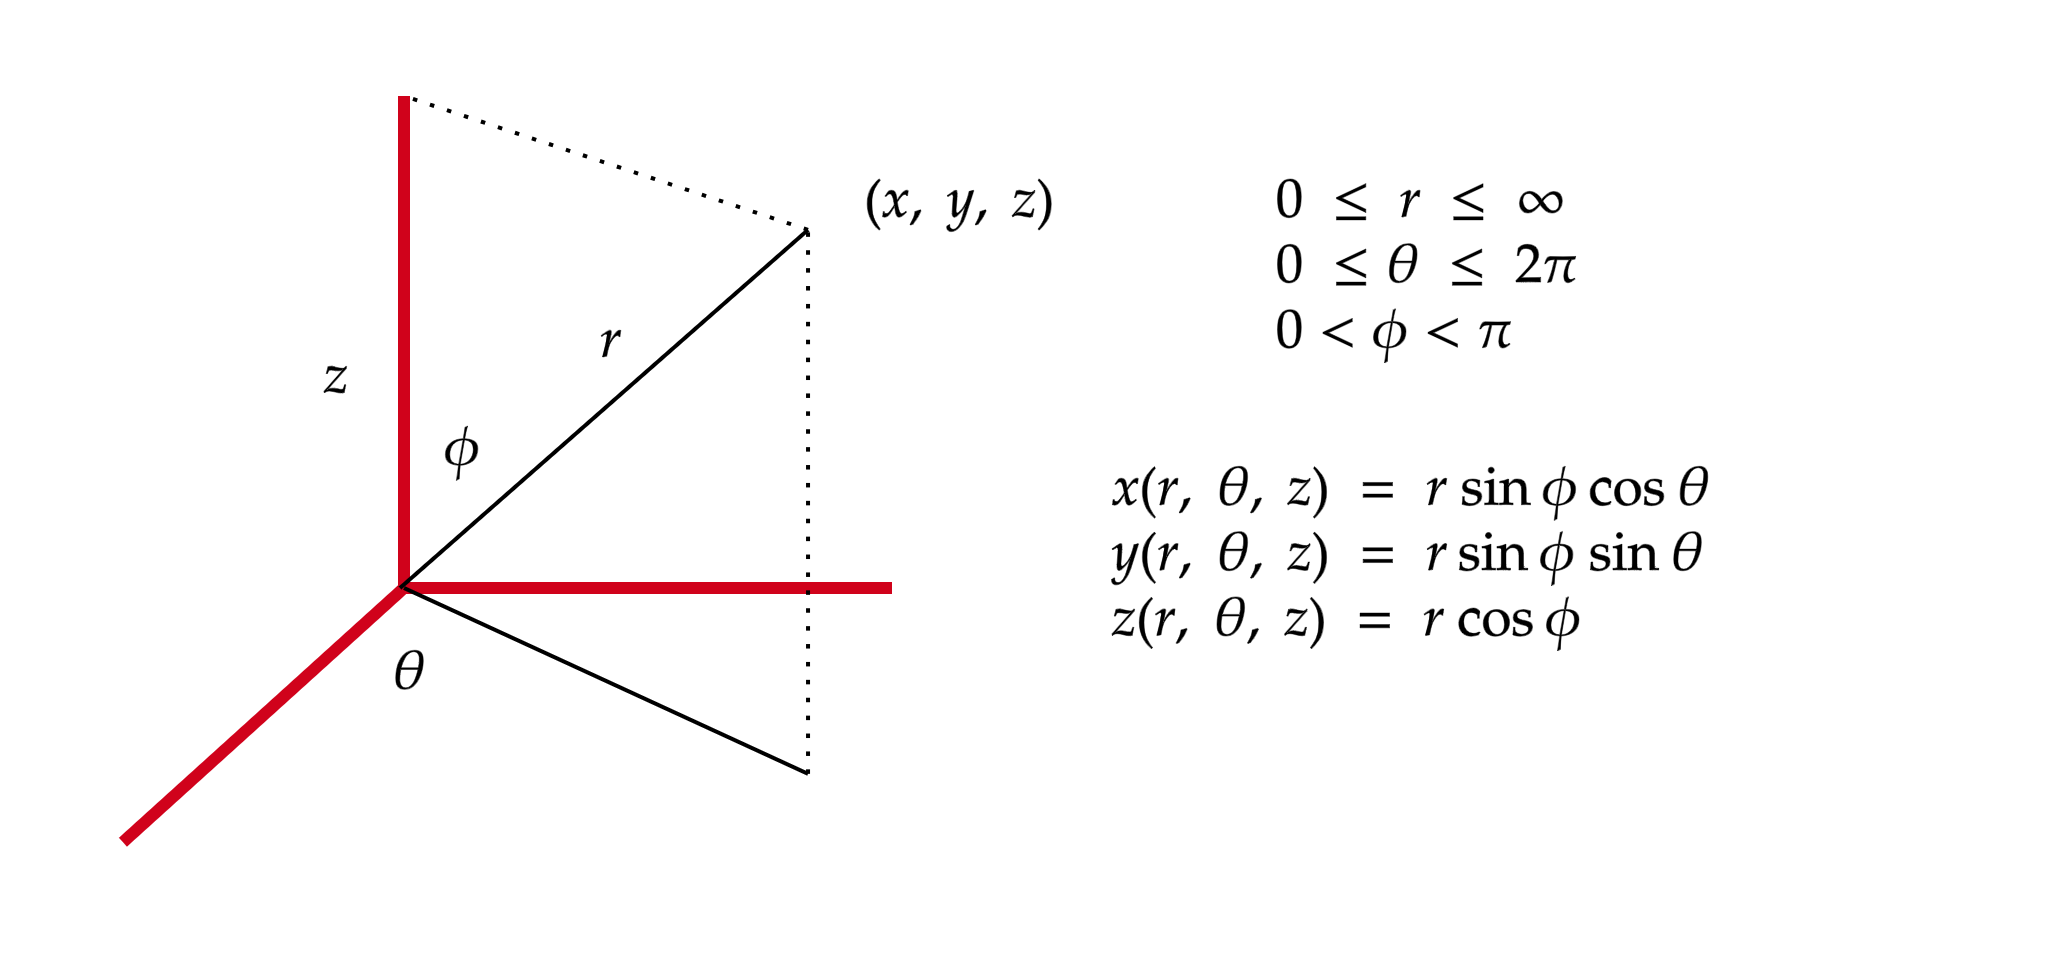
\includegraphics[width=0.7\linewidth]{figures/wk-6/fig-12.png}
\end{center}
with the determinant,
\begin{align*}
    \frac{\partial(x, y, z)}{\partial(r, \theta, \phi)}&=\operatorname{det}\left(\begin{array}{lll}
    x_n & x_\theta & x_{\phi} \\
    y_n & y_\gamma & y_{\phi} \\
    z_n & z_\theta & z_{\phi}
    \end{array}\right)
\end{align*}
which evaluates to,
\begin{align*}
    \left(\begin{array}{ccc}
    \sin \phi \cos \theta & -r \sin \phi \sin \theta & r \cos \phi \cos \theta \\
    \sin \phi \sin \theta & - \sin \phi \cos \phi & r \cos \phi \sin \theta \\
    \cos \phi & 0 & -r \sin \phi
    \end{array}\right)
    = -r^2 \sin \phi
\end{align*}

\begin{ex}{Two-Step Integration}{label}
    Let $a > 0$, $b > 0$, and $c > 0$. We will compute the integral,
    \[\iiint_A\left(\frac{x^2}{a^2}+\frac{y^2}{b^2}+\frac{c^2}{d^2}\right) d x d y d z\]
    where,
    \[A=\left\{(x, y, z) \in \mathbb{R} \mid \frac{x^2}{a^2}+\frac{y^2}{b^2}+\frac{z^2}{c^2} \leq 1\right\}\]
    We begin by defining the transformation,
    \[x = au \quad y = bv \quad z = cw\]
    so that,
    \[\frac{x^2}{a^2}+\frac{y^2}{b^2}+\frac{z^2}{c^2}=\frac{a^2 u^2}{a^2}+\frac{b^2 v^2}{a^2}+\frac{c^2 w^2}{c^2}\]
    Thus, $A^* = \{(u, v, w) \mid u^2 + v^2 + w^2 \leq 1\}$
    is a unit solid sphere. In particular,
    \[\frac{\partial(x, y, z)}{\partial(u, w, w)}=\operatorname{det}\left(\begin{array}{lll}
    a & 0 & 0 \\
    0 & b & 0 \\
    0 & 0 & c
    \end{array}\right)=a b c\]
    Putting everything together,
    \[\iiint_{A^*} (u^2 + v^2 + w^2) abc \cdot du dv dw\]
    evaluates to,
    \[\int_{\phi = 0}^{\phi = \pi} \int_{\theta = 0}^{\theta = 2\pi} \int_{r = 0}^{r = 1} r^4 \sin \phi dr d\theta d\phi = abc \cdot \frac{4 \pi}{5}\]
\end{ex}